\chapter{アンカーの発話区間検出実験}
\label{chapter:get_anchor}

\section{実験条件}
i-vectorの抽出には、ALIZEとLIR RAL\cite{alize}を用いる。i-vectorの抽出に使用するUBMモデルの学習には読み上げ音声\cite{ATR}を使用する。読み上げ音声に収録されている各発話データからi-vectorを抽出する。発話データから抽出する音響特徴パラメータを表\ref{iv_feature2}に示す。また混合数は32とした。\par

\begin{table}[H]
  \begin{center}
    \caption{使用する音響特徴パラメータ \label{iv_feature2}}
    \begin{tabular}{|c||c|} \hline
      特徴量 & 次元数\\ \hline
      MFCC & 19  \\ 
      POW & 1  \\ 
      $\Delta$MFCC & 19 \\ 
      $\Delta$POW & 1 \\ 
      $\Delta\Delta$MFCC & 19 \\ 
      $\Delta\Delta$POW & 1 \\ \hline
      計 & 60 \\ \hline
    \end{tabular}
  \end{center}
\end{table}

\noindent{\textbf{\underline{学習データ}}\par
UBMモデルの学習データに読み上げ音声\cite{ATR}を使用した。

\vspace{0.2in}\noindent{\textbf{\underline{評価データ}}}\par
「音声」の音源ラベルと発話の書き起こしが付与されているニュース番組5番組分を用いてアンカーの発話区間検出を行う。ニュース番組音声の詳細を表\ref{table:test_detail}に示す。また、ニュース番組5番組分に音源識別を用いて検出した発話区間の詳細を\ref{table:num_of_anchor}に示す。音源識別の詳細は付録\ref{section:devide_audio}に記載する。

\begin{table}[H]
  \begin{center}
    \caption{評価データの詳細 \label{table:test_detail}}
    \begin{tabular}{|c||c|c|c|} \hline
ニュースID & アンカー数 & 発話区間数 & アンカーの発話区間数 \\ \hline
ニュース1  & 1 & 345 & 165 \\ \hline
ニュース2  & 2 & 519 & 149 \\ \hline
ニュース3  & 2 & 608 & 258 \\ \hline
ニュース4  & 2 & 518 & 219 \\ \hline
ニュース5  & 2 & 520 & 285 \\ \hline
    \end{tabular}
  \end{center}
\end{table}

\begin{table}[H]
  \begin{center}
    \caption{検出した発話区間数とアンカーの発話区間数 \label{table:num_of_anchor}}
    \begin{tabular}{|c||c|c|} \hline
ニュースID & 発話区間数 & アンカーの発話区間数 \\ \hline
ニュース1  & 345   & 165 \\ \hline
ニュース2  & 519   & 149 \\ \hline
ニュース3  & 608   & 258 \\ \hline
ニュース4  & 518   & 219 \\ \hline
ニュース5  & 520   & 285 \\ \hline
    \end{tabular}
  \end{center}
\end{table}

\chapter{i-vectorの抽出精度向上のための発話区間結合手法}
\label{chapter:prob_method}
i-vectorを用いたアンカーの発話区間検出精度、音声認識精度は共にi-vectorの抽出精度によって大きく左右される。そこで、i-vector抽出精度向上のためにニュース番組特有の特徴である「対話表現が少ない」「同じ話者が連続で発話する」「様々な場所で発話する」の3点に着目した。これは、同じ話者の発話区間であると考えられる前後の発話区間を結合し、擬似的に長い発話を作成することでi-vectorの抽出精度の向上が見込めると考えたためである。そのため本稿では、2通りの方法で前後の同一話者と考えられる発話区間を結合する。1つ目は発話間の時間情報を考慮した発話区間の結合手法である。2つめは、話者の発話環境を考慮した発話区間の結合手法である。図\ref{fig:indexing2}は、本稿の提案手法を組み込んだインデクシング手法の流れである。

\begin{figure}[H]
  \begin{center}
    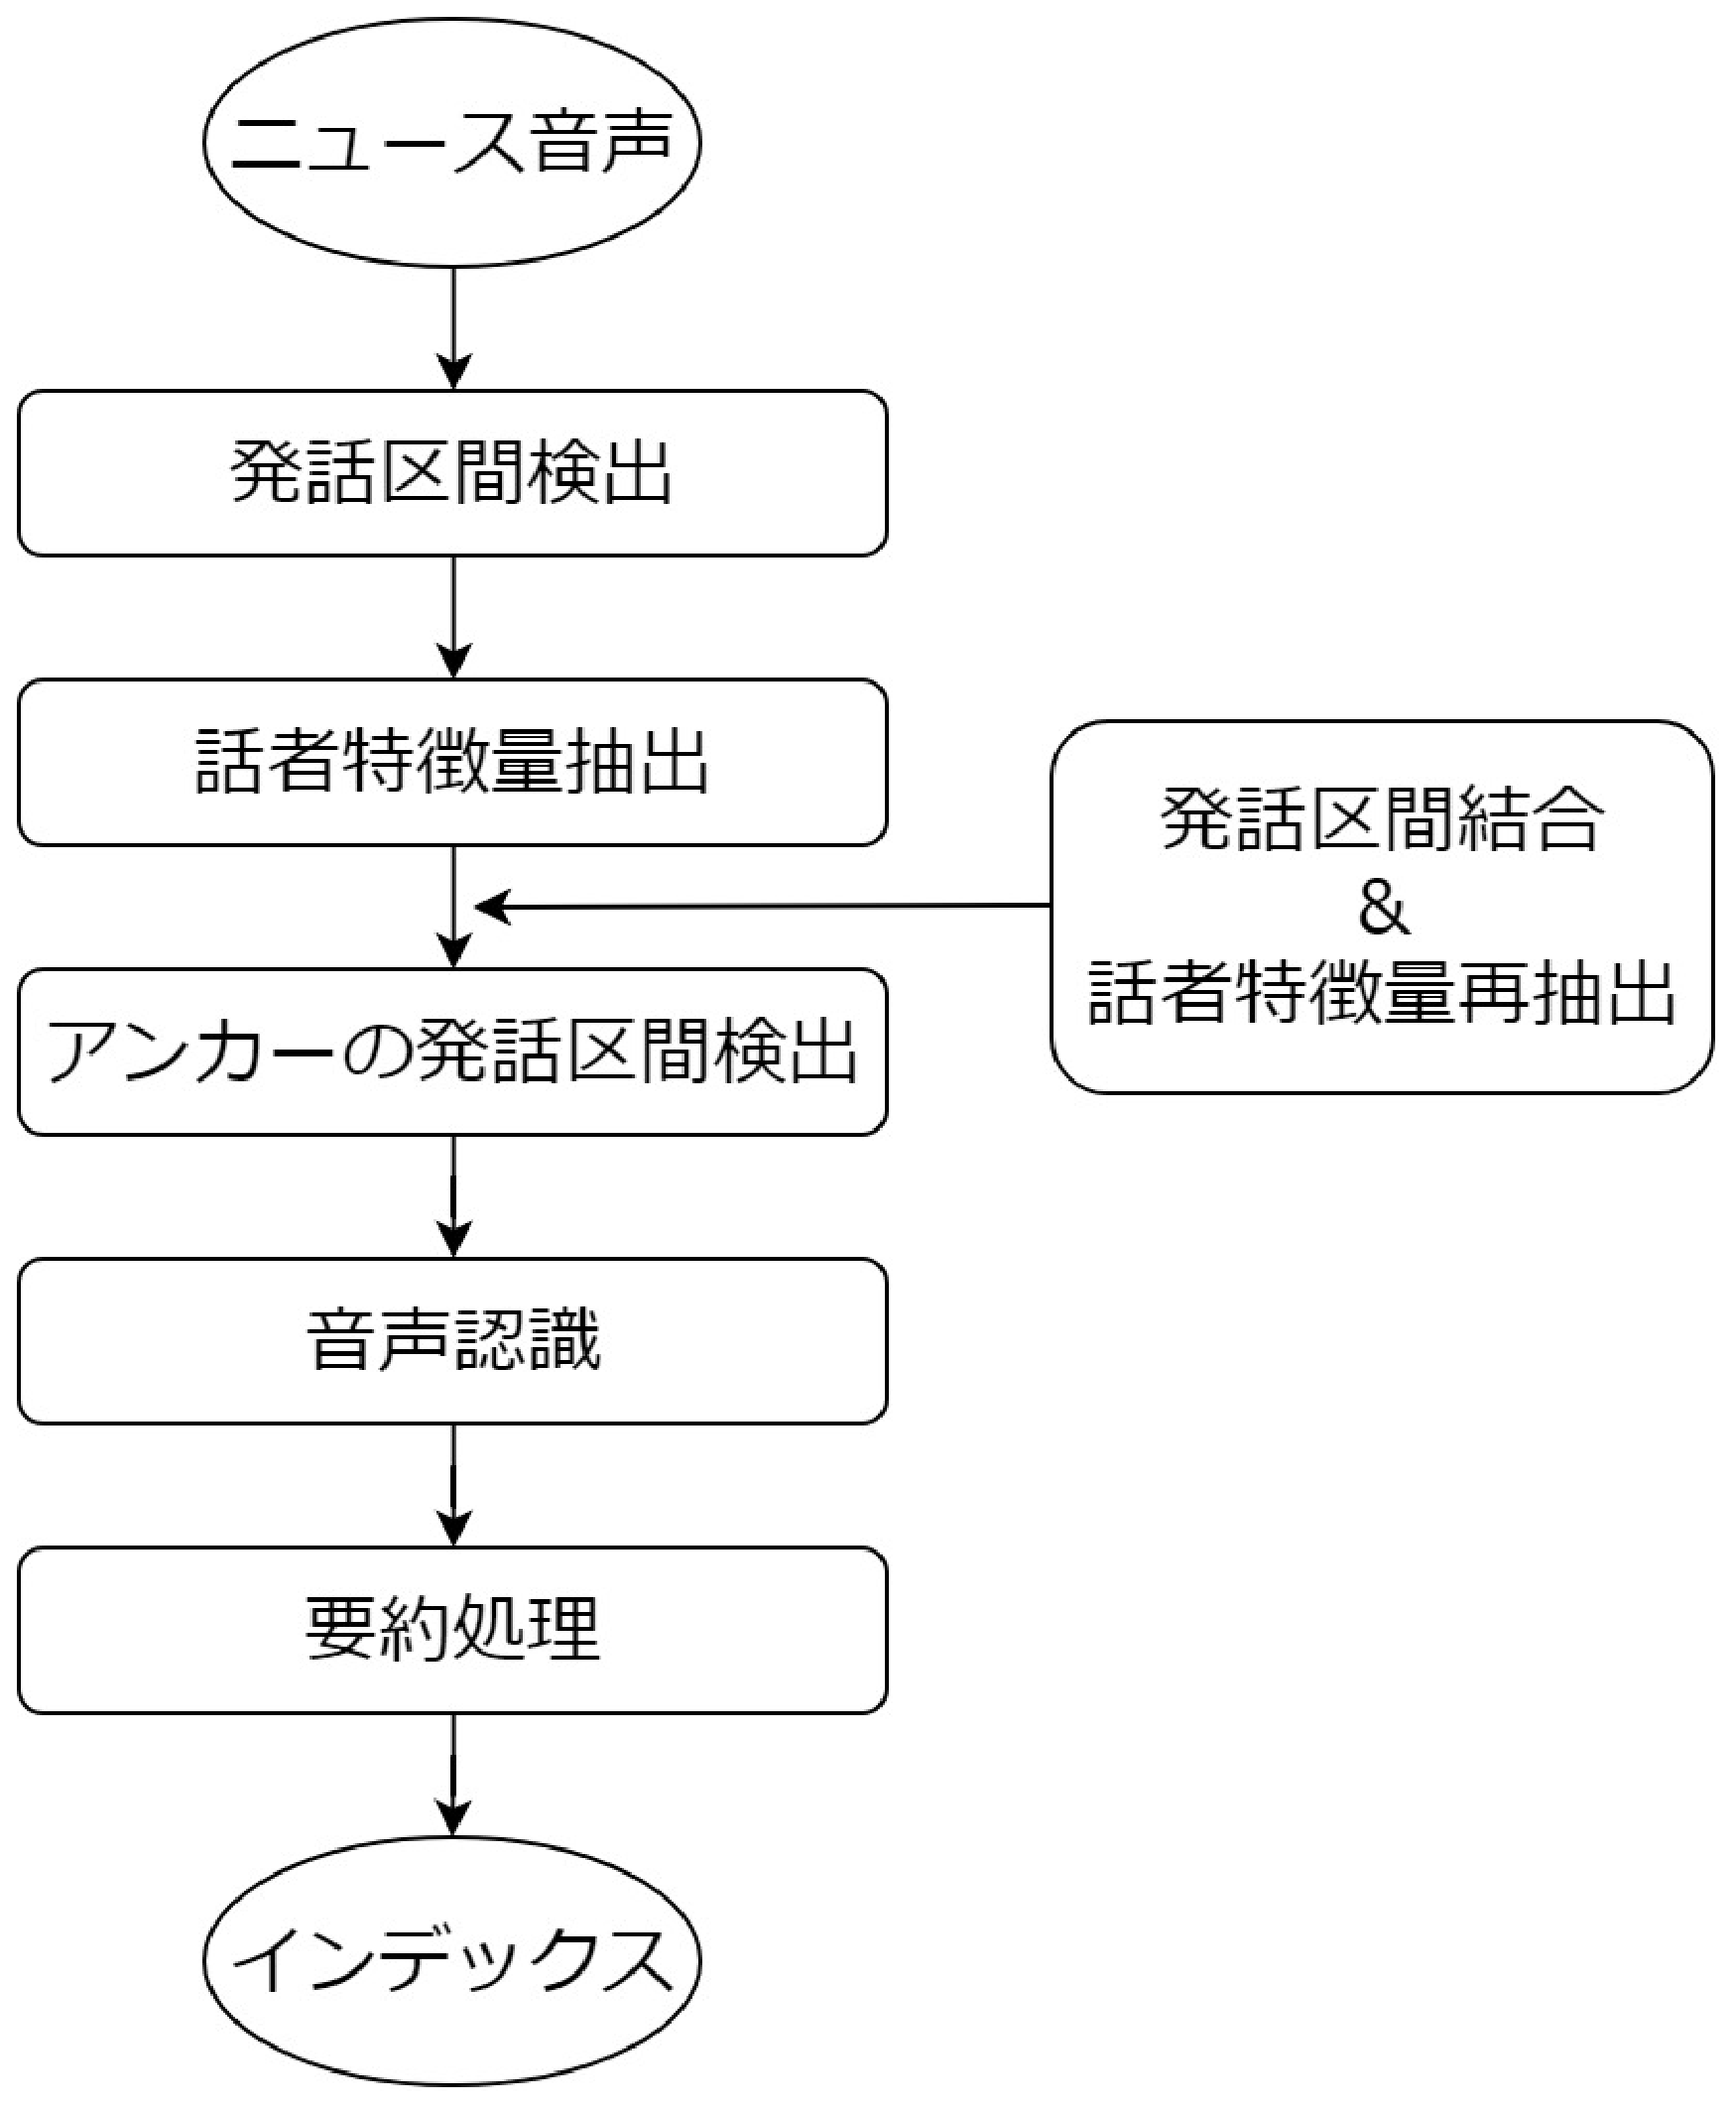
\includegraphics[scale=0.3]{./figure/indexing2.eps}
  \end{center}
  \caption{提案手法を組み込んだインデクシング手法 \label{fig:indexing2}}
\end{figure}

\section{発話間の時間情報を考慮した発話区間の結合手法}
本手法では、発話区間と発話区間の間(非発話区間)が短い場合、発話区間を結合する。これは図\ref{fig:same_sp}で示されるように、同一話者が連続で発話する場合は間をおかずに次の発話を行うことが非常に多いためである。つまり、非発話区間が非常に短いとき、高い確率で同一話者の発話が行われる。そこで、非発話区間が非常に短い場合、同一話者の発話と判別し発話区間を結合する。しかし、\ref{fig:different_sp}でもあるように、話者が切り替わった場合でも非発話区間が短い場合がある。このため、非発話区間の長さのみで結合した場合、異なる話者同士で発話区間を結合してしまい、i-vectorの抽出に悪影響がある。そこで、コサイン類似度の閾値$Th_{cos}$を設ける。非発話区間が非常に短く、その非発話区間を挟んでいる発話区間から抽出したi-vectorのコサイン類似度が一定値以上の時、同一話者同士の発話区間であるとして発話区間を結合する。

\section{発話環境を考慮した発話区間の結合手法}
本手法では発話環境を音源識別によって検出し、発話環境の変化を検出した場合、同一話者の可能性が高いとして前後の発話区間を結合する。ニュース番組にはスタジオにいるアンカーのほか、台風の状況を中継する中継アナウンサー、騒音の中でインタビューを受けるインタビューイなどが存在する。例えば、アンカーから中継アナウンサー、インタビューイからアンカーなど話者が切り替わった場合、発話環境が変化する。本稿で使用する音源識別システムはニュース番組音声を「音声」「背景雑音」「音楽」「無音」のいずれかに分類する。そのため、「音声」以外の区間、つまり非発話区間の音源識別結果である「背景雑音」「音楽」「無音」の検出結果が変化した時発話環境の変化したと識別することができる。以上の理由により、発話環境が変化するまでの範囲で発話している話者を同一話者として発話区間を結合する。\par


\section{i-vectorを用いたアンカーの発話区間検出手法\cite{nozaki_gakuseikai}}
\label{section:clustering}
アンカーの発話区間検出のために、i-vectorを用いて話者クラスタを作成し、クラスタに含まれる発話が多いクラスタをアンカーのクラスタとして発話区間を検出した。従来は話者クラスタの作成にk-meansが多く用いられていたが、ニュース番組ではアンカー以外にインタビューイ(インタビューの受け手)や中継の有無によって話者数が大きく異なるため、
あらかじめクラスタ数を決定する必要があるk-meansクラスタリングを用いることは適切ではないと考えた。そのため、アンカーの発話数は非アンカーと比較して多いことと、i-vectorはベクトル空間上で話者ごとに局所的に分布することに着目た。多くの発話のi-vectorが局所的に分布している部分のみをクラスタリングすることで、同一アンカーの発話区間を検出する。\par
本手法では、2つの発話データのi-vectorのコサイン類似度が閾値$Th_{cos}$以上の場合、その2つの発話データの話者は同一話者であると仮定した。まず、全ての発話データ間のi-vectorのコサイン類似度を求める。次に、このコサイン類似度が閾値$Th_{cos}$以上となる発話データ数が最も多い発話データを同一アンカーの発話データ群$O$のセントロイドとし、閾値$Th_{cos}$以上(話者性が類似している)の全データをそのデータ群$O$の初期要素とする。一方、i-vectorを抽出する発話データの発声の抑揚が大きい場合、同一話者の発話間のi-vectorであってもコサイン類似度が閾値$Th_{cos}$以下になる場合がある。そこで、発話データ$u_i(\in O)$と発話データ群$O$の距離が一定距離以内であるとき、発話データ$u_i$は発話データ群$O$の要素として追加する。以上の手順を繰り返してクラスタリングを行い、クラスタに含まれる発話が一定数以下となった時、クラスタリングを終了する。\par

\section{実験方法}
同一話者の可能性が高い発話区間を結合し、結合した発話区間からi-vectorを再抽出した。次に、再抽出したi-vectorを用いてアンカーの発話区間検出を行った。発話区間の結合手法は以下の通りである。

\begin{itemize}
\item 手法1 : 前後の発話のi-vectorのコサイン類似度と発話の間隔情報を考慮して発話区間の結合する
\item 手法2 : 前後の発話のi-vectorのコサイン類似度と発話環境を考慮して発話区間の結合する
\item 手法3 : 手法1 + 手法2
\end{itemize}

また、Baselineとして、音源識別によって得られた各発話区間から抽出したi-vectorを用いてアンカーの発話区間検出を行う。


前後の発話区間を結合する際のi-vectorのコサイン類似度の閾値を表\ref{table:decide_thcos}に示す。ここで、$T$は発話区間の秒数である。これは、図\ref{fig:same_cos_hist}で示されるように、同一話者間の発話であっても発話の長さによってコサイン類似度の値が大きく異なり、図\ref{fig:same_cos_vari}で示されるように発話が短い時、同一話者間のi-vectorのコサイン類似度の標準偏差が非常に大きいためである。そのため、本実験では、3.5秒と7秒で閾値を変更し、発話区間の結合に用いた。

\begin{table}[H]
  \begin{center}
    \caption{発話区間の結合の閾値 \label{table:decide_thcos}}
    \begin{tabular}{|c||c|} \hline
時間条件 & コサイン類似度の閾値  \\ \hline
$T <$ 3.5 &  0.2 \\ \hline
3.5 $\leqq T <$ 7 &  0.6  \\ \hline
7 $\leqq T$ &  0.75 \\ \hline
    \end{tabular}
  \end{center}
\end{table}

手法1、および手法3で用いる非発話区間の長さの閾値$Th_{time}$は0.8秒から1.5秒までの範囲を0.1秒刻みで行う。これは、図\ref{fig:same_sp}で示されているように、同一話者間の非発話区間が約1秒前後の長さを取ることが多く、図\ref{fig:different_sp},図\ref{fig:different_sp2}で示されているように、異なる話者間の非発話区間の割合が低いためである。\par
i-vectorを用いたアンカーの発話区間検出におけるアンカーか否かを判別する$Th_{cos}$は、先行研究\cite{nozaki_gakuseikai}と同様に0.5から0.8までの範囲を0.1刻みで変更して実験を行う。\par


\section{評価方法}
評価は、検出されたアンカーの発話区間と正解ラベルを比較して行う。

\begin{table}[H]
\begin{center}
    \caption{アンカーの発話区間の正誤判定 \label{table:clustering}}
\begin{tabular}{|c|c|c|c|l}
\cline{1-4}
\multicolumn{2}{|c|}{\multirow{2}{*}{}} & \multicolumn{2}{c|}{「発話者」のラベルが付与された発話区間} &  \\ \cline{3-4}
\multicolumn{2}{|c|}{}                  & アンカーの発話区間        & アンカー以外の発話区間        &  \\ \cline{1-4}
\multirow{2}{*}{判定結果}        & 正        & $TP$                  & $FP$                   &  \\ \cline{2-4}
& 誤        & $FN$                  & $TN$                   &  \\ \cline{1-4}
\end{tabular}
\end{center}
\end{table}

表\ref{table:clustering}に示すアンカーの発話区間の正誤判定を行い、$P$(適合率(Precision))と$R$(再現率(Recall))を式\ref{calc:precision2}と式\ref{calc:recall2}のようにそれぞれ計算する。また、$F$値($F-measure$)を式\ref{calc:fmeasure}のように計算する。

\begin{equation}
\label{calc:precision2}
P = \frac{TP}{TP + FP}
\end{equation}

\begin{equation}
\label{calc:recall2}
R = \frac{TP}{TP + FN}
\end{equation}

ここで$P$と$R$はそれぞれ適合率、再現率を表す。適合率が高い値を取るとき、識別結果に含まれる「誤り」の割合が少ないことを示している。また再現率が高いとき、識別結果に「漏れ」が少ないことを示している。一般的に、再現率の高いシステムは適合率が低く、逆に適合率が高いシステムは再現率が低い傾向にある。評価指標が2つあるとどちらのシステムが優れているかの判断が難しいため、適合率と再現率の調和平均を取り、ひとつのスカラ値に変換したF値(F-measure)がある。

\begin{equation}
\label{calc:fmeasure}
F = \frac{2 \times P \times R}{P + R}
\end{equation}

また、検出したアンカーの発話区間を式\ref{calc:anchor_acc}を用いて評価する。

\begin{equation}
\label{calc:anchor_acc}
Acc_{time} = \frac{検出したアンカーの発話区間の時間数}{アンカーの発話区間の時間数}
\end{equation}

本実験では、評価指標として適合率、再現率、$F$値、$Acc_{time}$を用いる。

\section{実験結果}
$Th_{time}$を変更してアンカーの発話区間検出精度が最も高いF値を示した条件の結果を図\ref{fig:result_anchor_baseline} $\sim$ 図\ref{fig:result_anchor_prob3}に示す。その他の条件の結果は付録で記載する。また、図\ref{fig:result_anchor_baseline} $\sim$ 図\ref{fig:result_anchor_prob3}に示された結果の中で、最も高いF値をとった条件のときの各ニュース番組のアンカーの検出精度を表\ref{table:baseline_eachnews} $\sim$ 表\ref{table:prob3_eachnews}に示す。

\begin{figure}[H]
  \begin{center}
    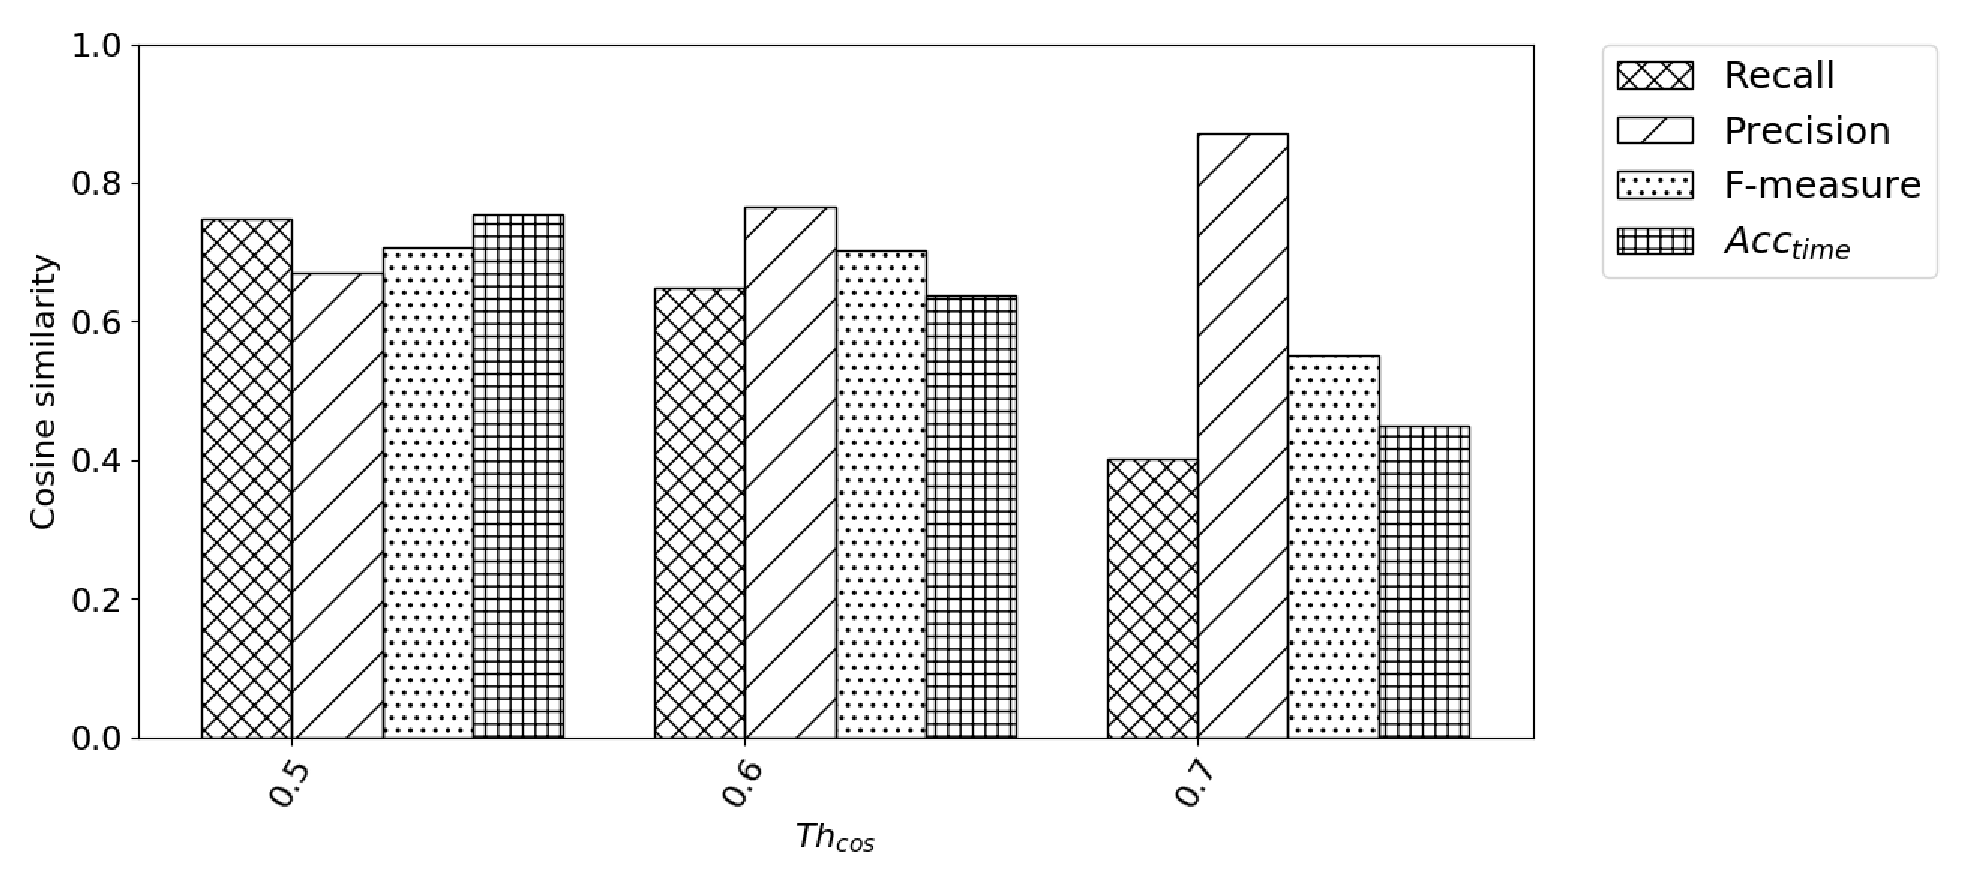
\includegraphics[scale=0.5]{./figure/baseline.eps}
  \end{center}
  \caption{Baselineによる発話区間検出精度 \label{fig:result_anchor_baseline}}
\end{figure}

\begin{table}[H]
  \begin{center}
    \caption{Baselineによる各ニュース番組音声のアンカーの発話区間検出精度($Th_{cos}=0.5$) \label{table:baseline_eachnews}}
    \begin{tabular}{|c||c|c|c|c|} \hline
データID & Recall & Precision & F-meature & 作成したクラスタ数\\ \hline
ニュース1 & 0.970 & 0.623 & 0.758 & 1 \\ \hline
ニュース2 & 0.709 & 0.437 & 0.540 & 2 \\ \hline
ニュース3 & 0.736 & 0.719 & 0.727 & 2 \\ \hline
ニュース4 & 0.728 & 0.661 & 0.693 & 2 \\ \hline
ニュース5 & 0.683 & 0.947 & 0.793 & 2 \\ \hline
    \end{tabular}
  \end{center}
\end{table}

\begin{figure}[H]
  \begin{center}
    \includegraphics[scale=0.5]{./figure/prob1_12.eps}
  \end{center}
  \caption{手法1によるアンカーの発話区間検出精度 ($Th_{time}=1.2$) \label{fig:result_anchor_prob1}}
\end{figure}

\begin{table}[H]
  \begin{center}
    \caption{手法1による各ニュース番組音声のアンカーの発話区間検出精度($Th_{cos}=0.6,Th_{time}=1.2$) }
    \begin{tabular}{|c||c|c|c|c|} \hline
データID & Recall & Precision & F-meature & 作成したクラスタ数\\ \hline
ニュース1 & 0.964 & 0.707 & 0.815 & 1 \\ \hline
ニュース2 & 0.764 & 0.685 & 0.722 & 2 \\ \hline
ニュース3 & 0.729 & 0.860 & 0.789 & 2 \\ \hline
ニュース4 & 0.683 & 0.741 & 0.711 & 2 \\ \hline
ニュース5 & 0.695 & 0.978 & 0.813 & 2 \\ \hline
    \end{tabular}
  \end{center}
\end{table}

\begin{figure}[H]
  \begin{center}
    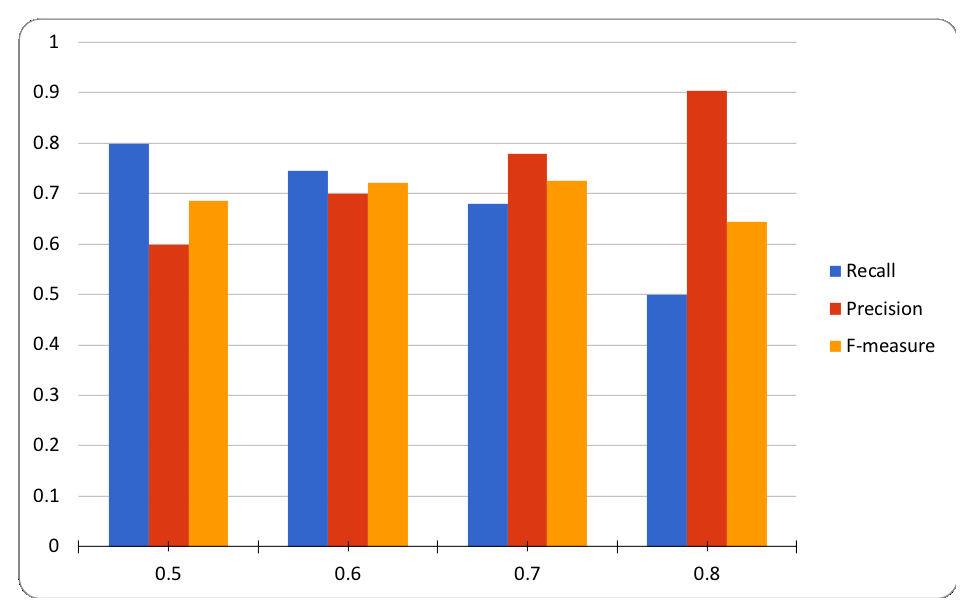
\includegraphics[scale=0.5]{./figure/prob2.eps}
  \end{center}
  \caption{手法2によるアンカーの発話区間検出精度 \label{fig:result_anchor_prob2}}
\end{figure}

\begin{table}[H]
  \begin{center}
    \caption{手法2による各ニュース番組音声のアンカーの発話区間検出精度($Th_{cos}=0.6$) }
    \begin{tabular}{|c||c|c|c|c|} \hline
データID & Recall & Precision & F-meature & 作成したクラスタ数\\ \hline
ニュース1 & 0.958 & 0.617 & 0.751 & 1 \\ \hline
ニュース2 & 0.788 & 0.512 & 0.621 & 2 \\ \hline
ニュース3 & 0.695 & 0.823 & 0.754 & 2 \\ \hline
ニュース4 & 0.683 & 0.732 & 0.707 & 2 \\ \hline
ニュース5 & 0.679 & 0.960 & 0.796 & 2 \\ \hline
    \end{tabular}
  \end{center}
\end{table}

\begin{figure}[H]
  \begin{center}
    \includegraphics[scale=0.5]{./figure/prob3_13.eps}
  \end{center}
  \caption{手法3によるアンカーの発話区間検出精度 ($Th_{time}=1.3$) \label{fig:result_anchor_prob3}}
\end{figure}

\begin{table}[H]
  \begin{center}
    \caption{手法3による各ニュース番組音声のアンカーの発話区間検出精度($Th_{cos}=0.6,Th_{time}=1.3$) \label{table:prob3_eachnews}}
    \begin{tabular}{|c||c|c|c|c|} \hline
データID & Recall & Precision & F-meature & 作成したクラスタ数\\ \hline
ニュース1 & 0.958 & 0.702 & 0.810 & 1 \\ \hline
ニュース2 & 0.758 & 0.590 & 0.663 & 2 \\ \hline
ニュース3 & 0.725 & 0.846 & 0.781 & 2 \\ \hline
ニュース4 & 0.646 & 0.755 & 0.696 & 2 \\ \hline
ニュース5 & 0.683 & 0.973 & 0.802 & 2 \\ \hline
    \end{tabular}
  \end{center}
\end{table}

実験の結果、発話区間を結合して再抽出したi-vectorを用いた手法が全体的に高い精度を示した。Baselineは$Th_{cos}$が0.8のときアンカーの発話区間を検出できなかった。また、Baselineは$Th_{cos}$が0.5のときがF-measureが最も高い値をとるのに対して、本提案手法では$Th_{cos}$が0.6のとき、F-measureが最も高い値をとった。\par
本実験の提案手法では、手法1が最も発話区間検出精度が高く、F値が0.772であった。また、いずれの手法においても$Th_{cos}$が小さい時にはRecallが高く、大きい時にはPrecisionが高くなる傾向が確認された。\par
殆どの手法でニュース2のアンカーの発話区間検出精度が最も低くなった。

\section{考察}
Baselineと再抽出したi-vectorを用いた各提案手法を比較したときアンカーの発話区間検出精度が向上したことから、従来と比較してi-vectorが話者の特徴をより抽出できたと考えられる。また、いずれの手法でもニュース2はアンカーの発話区間検出の精度が他のニュースと比較して低い。これは、アンカーの発話の割合が少ないためであると考えられる。それによって、インタビューイや天気アナウンサーの割合が高くなり、アンカーの発話を検出することが難しかったと考えられる。\par
提案手法の中では手法1が最も高いF値を示し、手法2および手法3は手法1と比較してアンカーの発話区間検出精度が低下した。これは手法2において、アンカーが発話中に参考映像などの背景雑音、音楽が鳴った場合、発話環境の変化と誤認識してしまい、十分な長さの発話を結合できなかったためであると考えられる。
